\section{DataBean und DataProxy}
\todo{citeing} \citep{gamma_entwurfsmuster:_2009}
Input und Output der einzelnen Pipelinefilter ist ein einziges
Datenobjekt vom Typ \code{DataBean}. 
\index{DataBean}
\index{Klasse!DataBean}
\name{DataBean} ist nach dem Konzept der \name{JavaBeans}
\footnote{\todo{JavaBean wasdas?}}
entworfen und ist mit hierfür typischen Funkionalitäten wie Serialisierung und
öffentlicher getter und setter Methoden ausgestattet.
\index{JavaBean}
\name{DataBean} bietet den Steps der Pipeline die Möglichkeit, ihre
(Zwischen-)Ergebnisse zentral abzuspeichern.
Die zu annotierende Inputsequenz \todo{name?} ist dabei ebenfalls Teilmenge der
von \name{DataBean} gespeicherten Daten.

Da es nur ein einziges Objekt vom Typ \code{DataBean} geben soll, das zentral
und für jeden Step innerhalb der Pipeline verfügbar ist, wird der Zugriff auf
dieses Objekt an einen Proxy
\footnote{\todo{proxy pattern? \citep{freeman_entwursmuster_2005}}}
delegiert.
Dieser übernimmt zudem die Implementierung einer geeigneten
Serialisierungsstrategie und synchronisiert die Zugriffe auf das
dahinterliegende \todo{doofes wort} \name{DataBean}.
Durch den Proxy ist die kongrekte Implementierung der Datenhaltung
\todo{anderes Wort ?!} vom Rest der Pipeline getrennt und kann leicht verändert
werden.
So wäre es beispielsweise denkbar, die Daten nicht local in einem Java Objekt
abzuspeichern, sondern entfernt in einer Datenbank abzulegen. \todo{toller
satz -.-}

Der \name{DataProxy} ist innerhalb der Pipeline ein \name{Singleton}
\footnote{\todo{singleton pattern wasdas}}.
Eine Referenz auf \name{DataProxy} ist Input für jeden Step und enthält nach
dessen Ausführung auch den Output.
Der Zugriff durch die Steps soll daher per \name{call by reference} erfolgen.

\begin{figure}[htbp]
	\begin{center}
		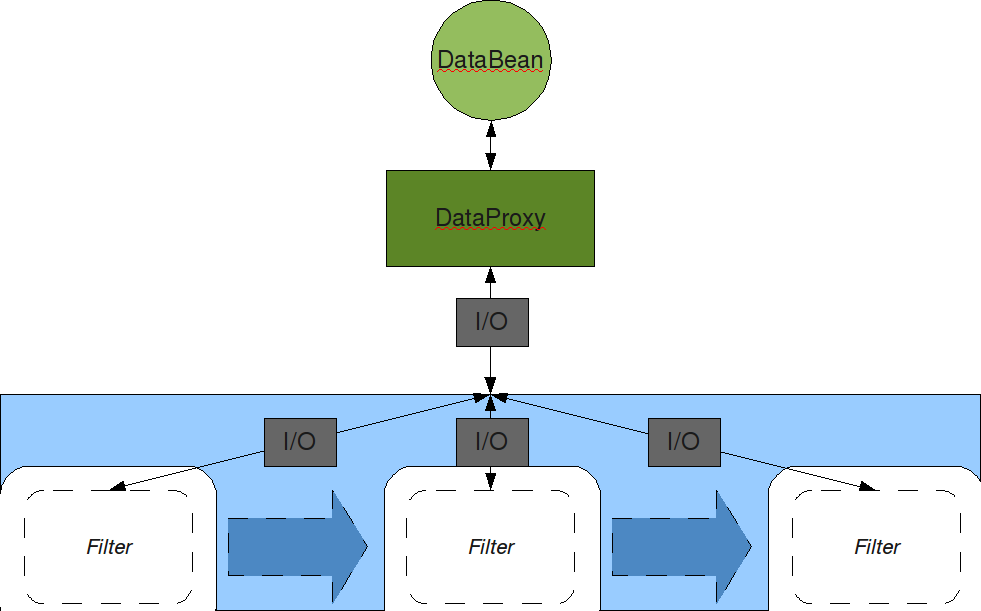
\includegraphics[scale=0.55]{pics/pipesFilter41.png}
	\caption[pipesFilter41]{
	\textbf{pipesFilter41.}
	something.}
	\end{center}
	\label{fig:pipesFilter41}
\end{figure}

\begin{figure}[htbp]
	\begin{center}
		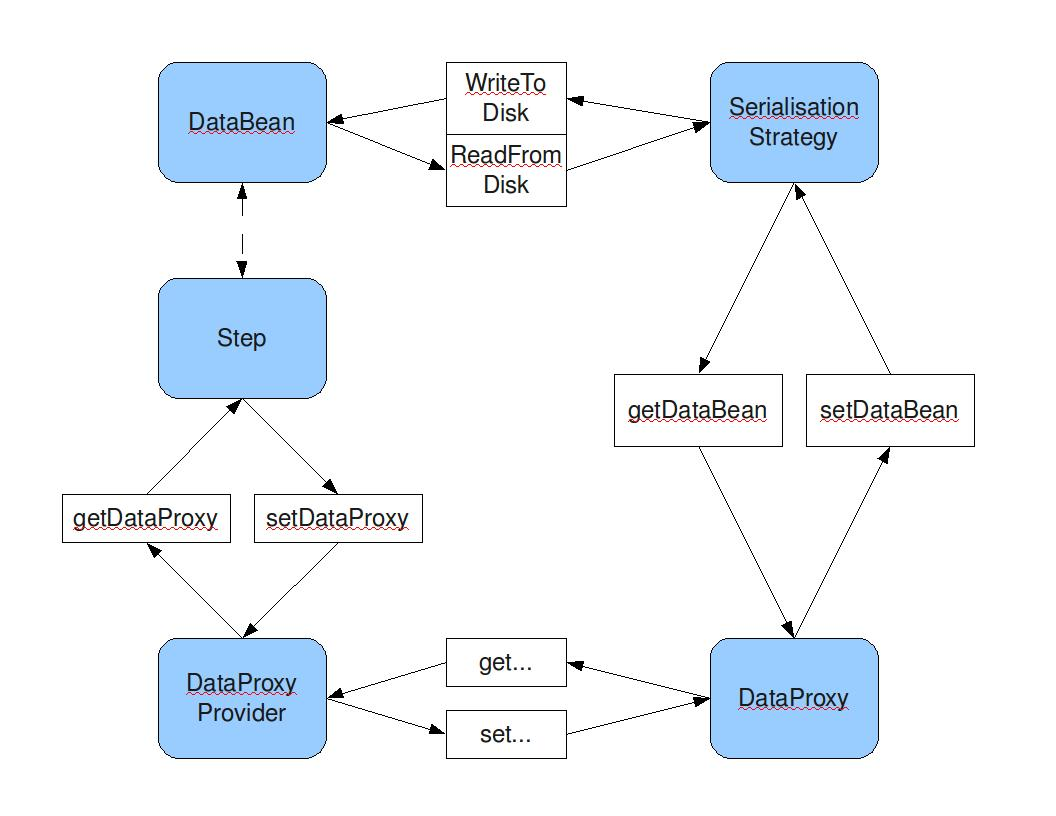
\includegraphics[scale=0.42]{pics/programDataManagment.jpg}
	\caption[Data Management]{
	\textbf{Data Management.}
	something}
	\end{center}
	\label{fig:programDataManagment}
\end{figure}